\chapter{Basic principles of Kubernetes}
\section{Container advantages over virtual machines}
In previous semesters we have already been able to gain initial experience with virtual machines (VMs) and also Docker containers regarding their architectural differences; if these terms and their architecture are not familiar to you, you can refer to Figure~\ref{fig:VM} and~\ref{fig:Container} to get in touch with them again before exploring minor details in the next section. 

    \begin{figure}[h]
        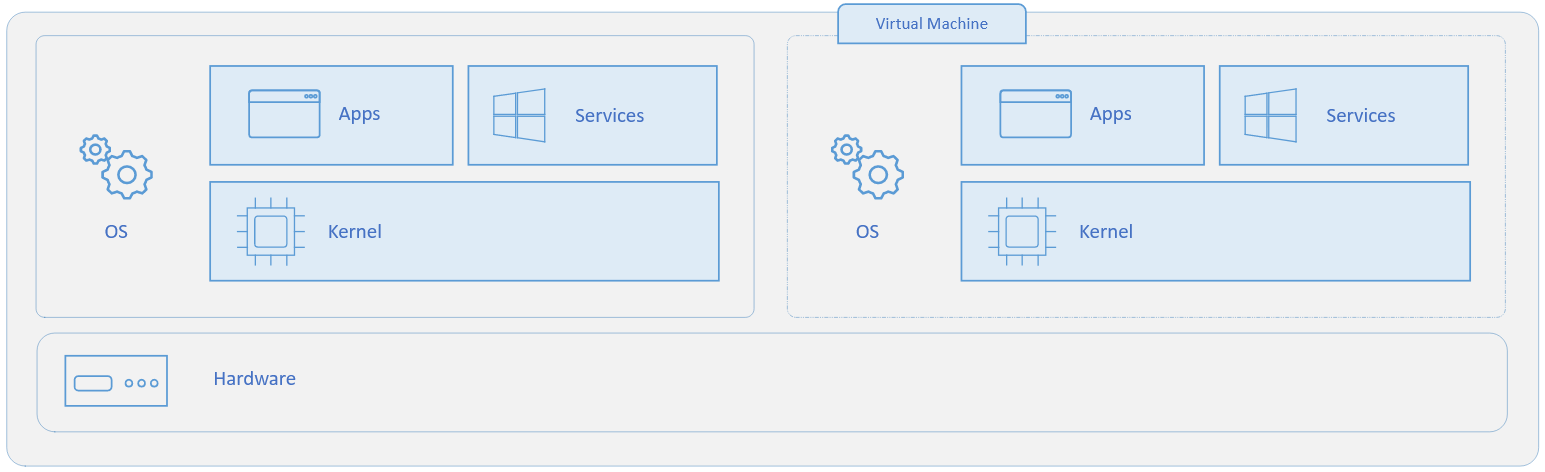
\includegraphics[width=15cm]{Bilder/VM.PNG}
            \centering
            \captionsetup{justification=centering, margin=1cm}
            \caption{Common virtual machine architecture.\cite{Microsoft:2021}}
            \label{fig:VM}
        \end{figure}

        \begin{figure}[h]
        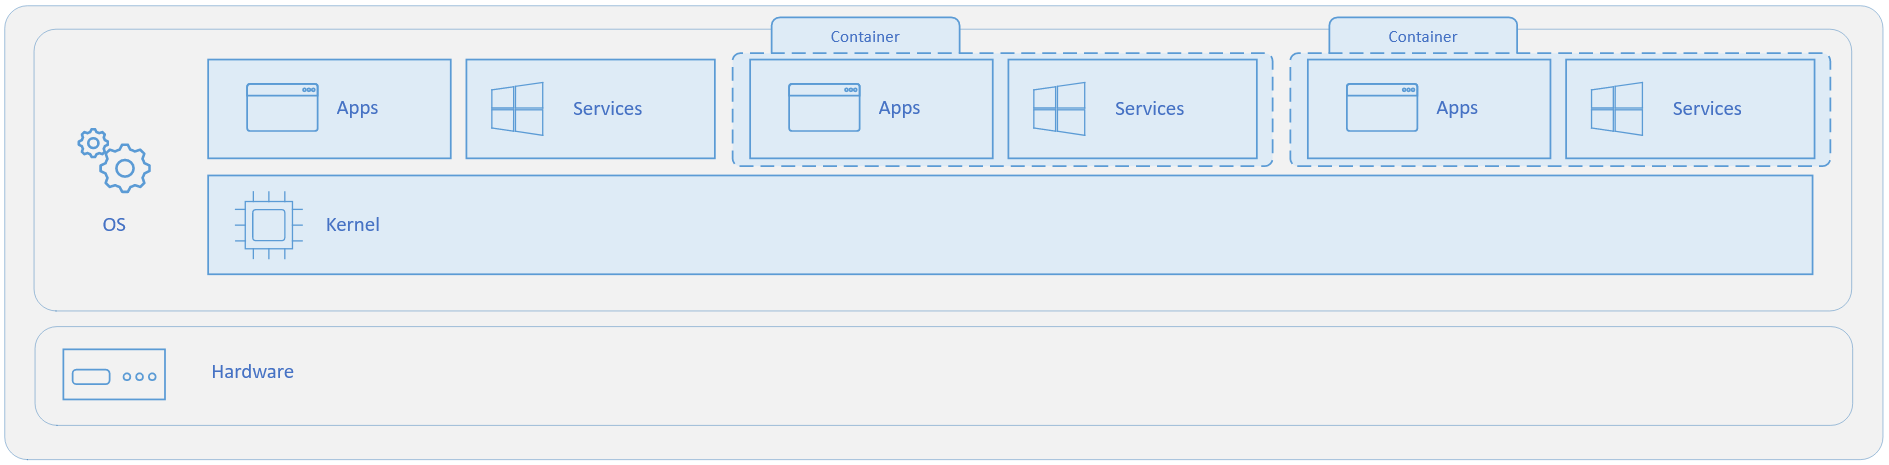
\includegraphics[width=15cm]{Bilder/Container.PNG}
            \centering
            \captionsetup{justification=centering, margin=1cm}
            \caption{Common container architecture.\cite{Microsoft:2021}}
            \label{fig:Container}
        \end{figure}

\subsection{Networking and isolation}
Virtual machines are exactly what you will expect hearing the term. Consequently each virtual machine is running a completely isolated operating system (OS) with its own kernel and dedicated CPU and storage on the underlying hardware. Since all hardware is virtualized, the network-adapter and network-infrastructure can be configured how you want it to be. Due to this, there is by default neither a connection to the host OS nor to other VMs set up on the system.\cite{Microsoft:2021}
\\\\Without further isolation methods like using Hyper-V isolation for containers, they just provide a lightweight isolation from the host and other containers. Hence they are less protected than default VMs but secure enough for most use cases. With regards to this lightweight approach mentioned before, one can say, containers are generally much more lightweight. For example referring to the system resource usage, each container can be tailored to just contain the needed services for the application running in it, leading to a lower system resource consumption compared to VMs. Likewise the networking functionality is implemented in a very lightweight way, causing a shared firewall for all containers with the host.\cite{Microsoft:2021}
\subsection{Load balancing and fault tolerance}
Load balancing is important to deal with fluctuating workloads, no matter whether it is about costumer purchases in a webshop or calculation a classification task. If you want to balance your load on VMs, you can only move them to other servers in a failover cluster. In contrast you would not move your containers by yourself, rather an orchestrator like Kubernetes will automatically start and stop containers on clusternodes (containing out of one or more servers) to manage changes in load. Further details on aforementioned orchestration by Kubernetes can be found in Chapter~\ref{sec:Advantages_Kubernetes}.\cite{Microsoft:2021}
\subsection{When to use containers over virtual machines - Summary}
In a nutshell containers are irreplaceable to work on a higher level of flexibility and auto\-mation. Due to the lightweight approach and their architecture, it is easier to handle containers in cloud environments and develop microservices with them. Application running in containers can be completely supervised by Kubernetes or other orchestrators helping you to get away from huge monolithic applications and passing on to these easily scalable microservice architecture structures. Another advantage of Containers (like e.g. Docker-Containers) is that they even virtualize their own operating system, giving you a freedom of choice where to deploy your services.\cite{Microsoft:2021,IBM:2021,SFL:2017}


\newpage\section{Advantages of Kuberenetes in containerization}
With many small containers running your applications or just parts of them, it can be quite challenging managing all of them and also to practice load balancing for better response times and better scalability. 
As mentioned before Kubernetes enables you to focus on developing your services instead of scaling the background architecture, starting up and shutting down your Containers and balancing your load. Although you need of course one or many capable systems with an appropriate amount of computing power for your service. Summarizing Kubernetes takes care of load balancing, resource management you. Furthermore in connection to other services like Grafana, one can use Kubernetes also as a monitoring source. \cite{Microsoft:2021,IBM:2021,SFL:2017,Cloud:2020,Kubernetes:2022} \label{sec:Advantages_Kubernetes}

%Cluster
\section{Kubernetes-Architecture}
The Kubernetes architecture is based on the principle of master and worker. In this context the Master is represented by the Masternode controlling all working instances called Workernodes. Further details according their cooperation will be introduced in the following sections. 
Besides the Term "Nodes" Kubernetes confronts you with terms like "Clusters" and "Pods". What they are and how they correlate with each other will also be explained to you in the next sections. Kubernetes can be quite complicated and is an abstract tool for advanced cloud service optimization therefore we just focus on main aspects of the tool.\cite{Ionos:2022}
\subsection{Pods}
Pods are the smallest deployable unit that can be created and managed in Kubernetes. A Pod contains usually one or under certain circumstances several running containers sharing storage and network resources. The main task of a Pod is modeling a logical server with the interdependent containers (in a Pod) running on it. This logical server running containers in a cloud environment can be compared to a physical server running applications. The resources used by a Pod remain always on the same (virtual) server and calculations inside this Pod are jointly planned and executed, such as the resources used by a standalone physical server also remain on its hard disk and calculations are only influenced by applications running on exactly this server.
\\\\Summarizing in terms of container concepts, a Kubernetes Pod is similar to a group of containers that share resources like namespaces and file system volumes.\cite{Kubernetes_pods:2022}
\newpage\subsection{Master- and Workernodes}
\textbf{Masternode:}
\\The Masternode controls the state of the cluster (which is explained in the next section), e.g. which applications are running. The master node is the starting point for all task assignments. It coordinates among others the following processes: Scheduling and scaling of applications, maintaining the state of a cluster and also implementing updates to applications running inside the Pods in Workernodes.\cite{Kubernetes_cluster}
\\\\\textbf{Workernode:}
A Kubernetes Workernode is a working machine in Kubernetes either represented by a VM or a physical machine. Each and every Workernode is orchestrated by the Masternode and contain the services needed to run the dedicated pods with its applications.  Furthermore the services on a node include the container runtime, the Kubelet, and the Kube proxy. The container runtime is installed in every node in the cluster so that Pods can run there. 
The container runtime is a program installed in every node in the cluster and is responsible for running the individual Pods. It must be compatible with both the Container Runtime Interface (CRI) and the Container Network Interface (CNI). CRI-O and containerd are two container runtime examples. A Kubelet interacts with the CRI, the default program for creating and managing containers, to ensure that containers in a pod are running and a Kube proxy manages network connectivity and maintains network rules across nodes. The Kube proxy implements the Kubernetes service concept at each node in a given cluster.\cite{Kubernetes_cluster, Kubernetes_nodes:2021, Kubernetes_runtime:2022}
\subsection{Clusters}
A Kubernetes Cluster is a group of nodes that run container-based applications. Those Clusters allow containers to run across multiple machines and in multiple environments: virtual, physical, cloud-based, and on-premises. Unlike virtual machines, Containers are not limited to a specific operating system, but can also work together running on various operation systems. A cluster also contains several services like:
    \begin{itemize}
        \item \textbf{API-Server:} Provides a REST-interface for all Kubernetes resources and serves as the frontend of the Kubernetes control plane.
        \item \textbf{Scheduler:} Places containers according to resource requirements and metrics. The scheduler also remembers which pods are currently not linked with any pod and selects sutable nodes on which to run those pods.
        \item \textbf{Controller-Manager:} This component executes controller processes and controls the state of the cluster with the desired specifications.
        \item \textbf{Etcd:} This component stores all cluster data. Etcd is a consistent and highly available Kubernetes backup store. 
    \end{itemize}

\noindent Besides that Kubernetes Clusters also contain a Kubelet and a Kube-Proxy working as the counterpart of the Kubelets and a Kube-Proxys in Nodes. Figure \ref{fig:Cluster} shows the architecture of a single Kubernetes Cluster with two Nodes (A and B). Node A contains two Pods and Node B contains one Pod. Up to three containers are running in these pods.\cite{Kubernetes_cluster}

    \begin{figure}[h]
        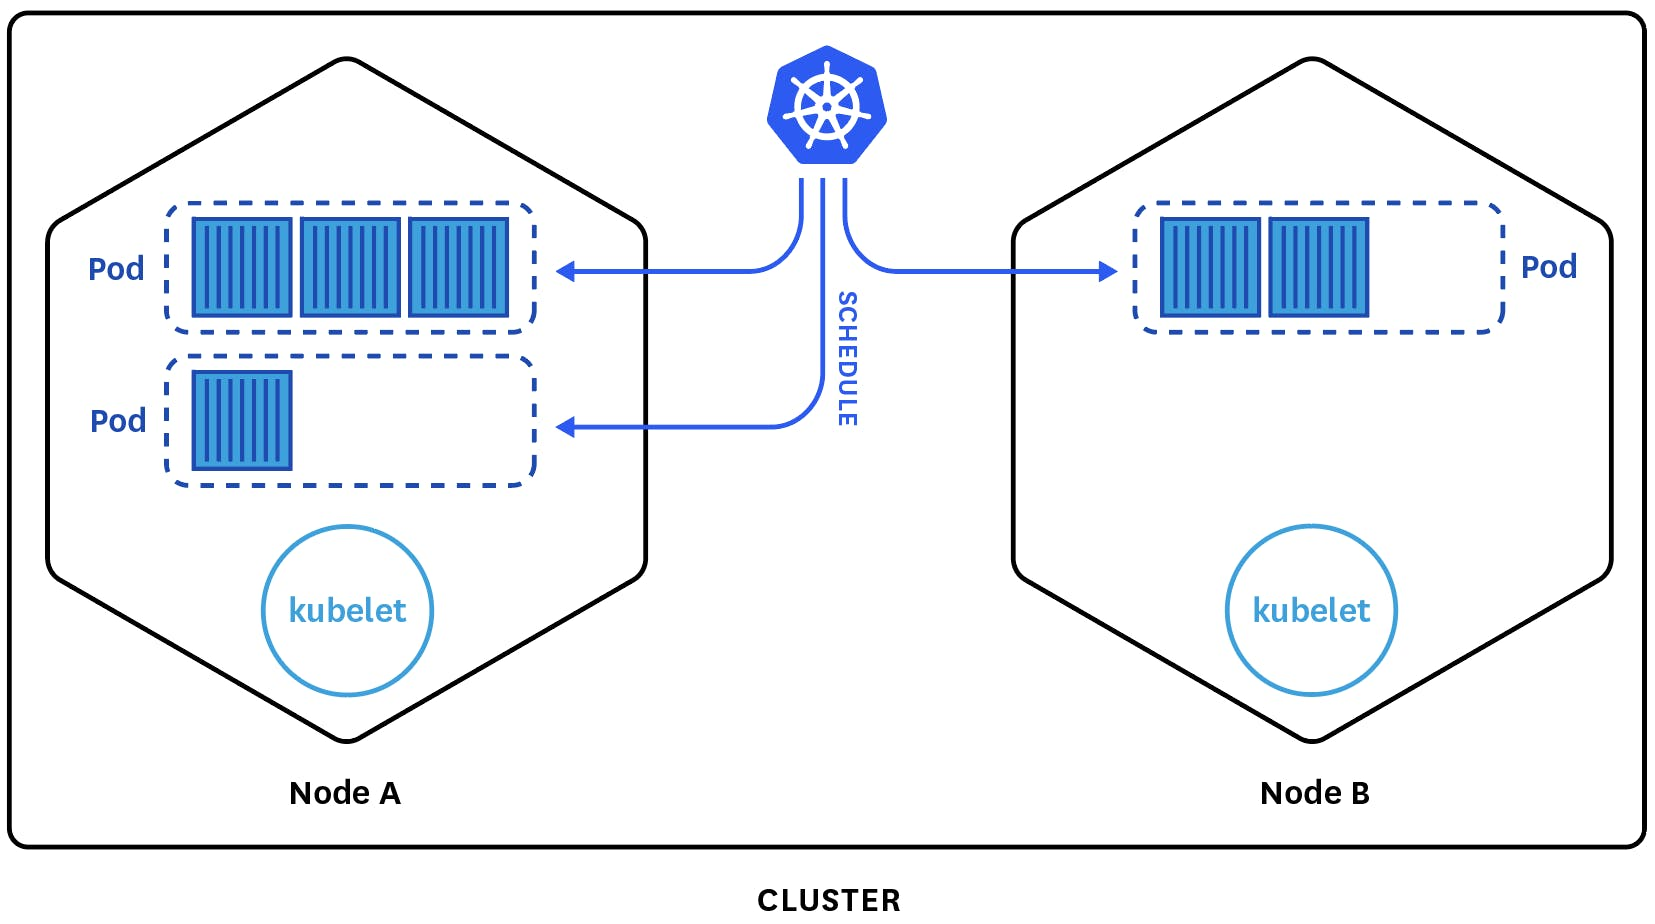
\includegraphics[width=15cm]{Bilder/kubernetes-pods.jpg}
            \centering
            \captionsetup{justification=centering, margin=1cm}
            \caption{Overview of a Kubernestes Cluster archtecture, the scheduler is represented by a Kubernetes icon.\cite{Datadog:2020}}
            \label{fig:Cluster}
        \end{figure}

\subsection{Networking}
Kubernetes uses a flat network model for communication within the cluster. Every Pod in a cluster receives its own unique cluster-wide IP address, which means you don't have to actively construct linkages between Pods, and you don't have to deal with mapping container ports to host ports very often. This results in an approach in which Pods may be treated similarly to VMs or physical hosts in terms of port allocation, name, service discovery, load balancing, application setup, and migration. The following two essential criteria are imposed by Kubernetes on any network implementation: 
\begin{itemize}
    \item pods can communicate with all other pods on any other node without NAT
    \item agents on a node (e.g. kubelet) can communicate with all pods on that node
\end{itemize}

\noindent This architecture is intended to choose simplicity overall, but it is also mostly compatible with Kubernetes objective to enable low-friction app transfer from VMs to containers. If your application previously ran in a VM, your VM had an IP-Adress and was able to communicate with other VMs in your project. This is the same basic model.
\\\\Containers within a Pod share their network namespaces, including their IP address and MAC address, hence Kubernetes IP addresses exist at the Pod level. This implies that containers within a Pod may all access each other's localhost ports. The exact implementation is a detail of the particular container runtime in use.\cite{Kubernetes_network:2022}